\documentclass[a4paper,12pt]{scrreprt} %A4, 12-Punkt-Schrift, science-report als stil.
\usepackage[justification=centering]{caption}

\usepackage{graphicx} %zum einfgen von bildern
\usepackage{url}%fr urls
\usepackage{fancyhdr} %fr kopf- und fusszeilen
\usepackage{setspace} %zeilenabstand
\usepackage{makeidx} %frs inhaltsverzeichnis
\usepackage{eurosym} %Frs Eurosymbol
%\usepackage[ngerman]{babel} %die drei zeilen sind fr umlaute, scharfes � anfhrungszeichen im deutsch-stil
%\usepackage{ngerman}
\usepackage[T1]{fontenc}
\usepackage[latin1]{inputenc}
\usepackage{longtable}%fr Tabelle ber mehrere Seiten
%\usepackage[nooneline,it]{caption2}
\usepackage{array} %fr Tabelle
\usepackage{geometry} %fr Seitengr�eneinstellungen
%\geometry{left=27mm,right=22mm,bottom=27mm,top=30mm,headsep=10mm,footskip=12mm}
\geometry{left=37mm,right=25mm,bottom=41mm,top=31mm,headsep=10mm,footskip=12mm}
%\usepackage{nofloat}%nicht flie�ende Tabellen und bilder
\usepackage{rotating} %fr Tabelle quer auf Blatt
\usepackage{colortbl}%damit (z.B) Zellen einer Tabelle farbig hinterlegt werden k�nen
\usepackage{color} %fr farbige W�ter
\usepackage{hhline}
\usepackage{supertabular}
\usepackage{fancybox} %fr Rahmen um Bild un Text
\usepackage{pifont} % fr Symbole
\usepackage{varioref}
\usepackage{booktabs}
\usepackage{dcolumn}
\usepackage{subfigure}
\usepackage{tabularx} %fr Tab mit fixer Breite
\usepackage{units}
\usepackage{multirow}
\usepackage{hvfloat}
\usepackage{cite}
\usepackage{amssymb,amsmath}
\usepackage{paralist}
\usepackage[pdftex,pdfauthor={Christoph Egger},pdftitle={BIQINI},colorlinks]{hyperref}
%fr input von source
\definecolor{hellgelb}{cmyk}{0,0,0.5,0}
\usepackage{listings}
\lstset{numbers=none, numberstyle=\tiny, numbersep=5pt,language=java,basicstyle=\scriptsize,breaklines=true,captionpos=b,frame=single}%,resetmargins=true}
\renewcommand{\labelitemi}{\symbol{45}}

\onehalfspacing %einenhalb-zeilenabstand

\renewcommand{\topfraction}{0.85}
\renewcommand{\textfraction}{.1}
\renewcommand{\floatpagefraction}{0.75}

\setlength{\parindent}{0pt} %eine einrckung der ersten zeile bei neuen abs�zen - wenn du eine einrckung willst, einfach nicht 0 reinschreiben.
\setlength{\parskip}{1 em} %Abstand zum n�hsten Absatz
%\setlength{\skip\footins}{5mm} %Abstand von Fussnote zum Text drber
\setlength{\footnotesep}{4mm} %Abstand zwischen Fussnoten

%Stil der Seite auf Fancy stellen
\pagestyle{fancy} 
\fancyhead{} %Kopfzeile
\fancyfoot{} %Fu�eilen
\renewcommand{\headrulewidth}{0.5pt} %Strich in der Kopfzeile
\renewcommand{\footrulewidth}{0.5pt} %Strich in der Fu�eile
\cfoot{\bfseries{\thepage}}%Seitenzahl in Fusszeile, Seitenmitte
\lhead{\nouppercase{\rightmark}}%Kopf rechts, Text nicht in Kapit�chen
%Stil fr Plain Seiten anpassen
\fancypagestyle{plain}{%Kopfzeile auch am Kapitelanfang
	\renewcommand{\rightmark}{}
	\fancyhead{}
	\fancyfoot{}%kopf- und fu�eilen
	\renewcommand{\headrulewidth}{0pt} %Strich in der Kopfzeile
	\renewcommand{\footrulewidth}{0.5pt} %Strich in der Fu�eile
	\cfoot{\bfseries{\thepage}}%Seitenzahl in Fusszeile, Seitenmitte
	\lhead{\nouppercase{\rightmark}}%Kopf rechts, Text nicht in Kapit�chen
}

%%%ACHTUNG%%%
\renewcommand{\arraystretch}{1.2}%Damit mehr Platz zwischen Text und Linie einer Tabelle ist.

%\setlength{\footskip}{0cm} %Abstand Unterkante Rumpf bis Unterkante Fu�eile
%\setlength{\textwidth}{455pt} %frs Binden muss der mittlere Teil (Text, Bilder, Tabellen usw.) weiter nach links
%\renewcommand{\headwidth}{\textwidth}
%\setlength{\hoffset}{6pt}
%\setlength{\textheight}{670pt} %Texth�e erh�en
%\usepackage{layout}
\makeindex
\begin{document}
 \begin{titlepage}
		\begin{center}
			\LARGE BIQINI\\
		%\end{flushleft}
		\vspace{3cm}
		%\begin{center}
			\Huge	\sf \textbf{BACCARDI IMS QOS IMPLEMENTATION INITIATIVE.}\\ \rm
			
			\vspace{7cm}
			\large Christoph Egger\\
			\large Marco Happenhofer\\
			\large Joachim Fabini\\
			\large Peter Reichl
			\vspace{1cm}
		\end{center}
		\normalsize
		\vfill
	\end{titlepage}
\tableofcontents
\chapter{Motivation}
Driven mainly by the high capacities available in fixed access networks, the imminent end-of-life of circuit-switched equipment, and the huge expectations concerning OPEX (operational expenses) reduction when operating one single IP- based platform, the replacement of circuit-switched voice networks by packet- switched data networks is currently experiencing a strong progress. However, the
architectural	requirements	of	such	large-scale	carrier-grade	IP-based telecommunication systems exceed the complexity of plain IETF SIP networks by orders of magnitude in order to enable satisfactory user experience already for the most important basic service, which is still voice. In this context, the IP Multimedia Subsystem (IMS), standardized by the 3rd Generation Partnership Project (3GPP), has become an important candidate architecture for the access-agnostic covering of all relevant aspects from signaling to media, from QoS reservation to security, charging and billing. Recently, several standardization bodies, namely 3GPP, 3GPP2, ETSI TISPAN and PacketCable, have joined their forces to define an interoperable Common IMS platform, agreeing to maintain one single set of 3GPP standards starting with 3GPP Release 9. Moreover, recognizing the need for interoperability and lower IMS complexity, main IMS vendors and operators have engaged in initiatives like One Voice and Rich Communication Suite Initiative (RCSI), defining minimum mandatory sets for IMS system- and service-level capabilities and features.

Released under the GNU Public License in 2006, the Fraunhofer FOKUS Open Source IP Multimedia Subsystem Core (OpenSource IMS) implementation has become a cornerstone of the scientific and industrial IMS research community. OpenSource IMS offers a generic, extensible 3GPP Release 7 IMS core network reference implementation, including signaling and security features as well as modules supporting the extension by means of additional interfaces (reference points). However, today's fixed and upcoming Next Generation Mobile Network (NGMN) access technologies and --services, which require network capacities exceeding the ones of existing 3G networks by an order of magnitude, mandate the use of adequate service-specific QoS enforcement mechanisms to maintain a Quality of Experience (QoE) similar to the one guaranteed by circuit-switched voice services. Despite of this urgent need, this function is not implemented by OpenSource IMS.

Therefore, this apparent gap has been addressed within the application-oriented project BACCARDI (Beyond Architectural Convergence: Charging, SeCurity, Applications, Realization and Demonstration of IMS over fixed and wireless networks) which has been conducted at the Telecommunications Research Center Vienna (FTW) during the years 2008 and 2009. As a result, the BACCARDI IMS QoS Implementation Initiative (BIQINI) has designed and implemented a QoS enforcement function which extends the OpenSource IMS by means of a generic, extensible, 3GPP Release 7 conforming Policy and Charging implementation and the corresponding interfaces. Main parts of the BIQINI concept and implementation have been contributed by the Institute of Broadband Communications (IBK), Vienna University of Technology, with support of FTW and the associated industry project partners Alcatel-Lucent Austria, Kapsch CarrierCom, mobilkom austria, and Telekom Austria.

The main aim of BIQINI is to provide a highly flexible QoS playground and multi- purpose plug-in for policy repositories, implementing a complex, stateful rules function, supporting active network capacity management as well as the PCC push model. With respect to this feature, BIQINI's Policy Enforcement component extends OpenSource IMS to become a reliable testing platform for Quality of Experience (QoE) for real-time multimedia streams. Note, however, that BIQINI
does not depend on OpenSource IMS, and instead supports integration with other SIP or non-SIP session-based signaling protocols as well.

In this document we argue that BIQINI provides a clear advancement compared to the current state of the art, most notably the open source Policy and Charging Control Framework (PCC) published by a group of the University of Capetown (UCT) in 2007. In contrast to BIQINI, the UCT PCC operation relies on stateless gate opening and closing, moreover its architectural framework is relatively limited with respect to scalability, extensibility and active link capacity management.

Within the open source community, in November 2009 the NGN working group of Fraunhofer FOKUS has announced an Evolved Packet Core (EPC) implementation which is supposed to include a PCC. However neither the detailed concept nor the implementation of the OpenEPC has been released so far.

To the best of our knowledge, these two contributions already conclude our account of current related work. In contrast, commercial PCC solutions are offered by various IMS vendors. However, two factors are prohibitive in deploying these implementations in applied IMS research at universities or other non-profit institutions: from a technical point of view, these implementations are closed source, which hinders additions and modifications at source code level, whereas the cost factor of PCRFs and particularly of PCEFs provides a huge barrier for IMS-related research activities.

%%%%%%%%%%%%%%%%%%%%%%%%%%%%%%%%%%%%%%%%%%%
\chapter{QoS Enforcement Architectures and Tools}
Having recognized that the promotion of three diverging IMS standards for mobile, fixed and cable networks, respectively, entails the severe danger of an overall IMS failure, 3GPP has agreed in 2007 together with other involved standards organizations, notably ETSI TISPAN for fixed networks and PacketCable for cable networks, to harmonize their corresponding standardization activities. Starting with 3GPP Release 8, the 3GPP therefore develops and promotes a Common IMS architecture which conforms to the requirements of all three standardization bodies, whereas in 3GPP Release 7, main QoS-related interfaces (reference points), particularly Rx/Gx for 3GPP and Gq'/Re for the Resource and Admission Control Subsystem (RACS), are not yet harmonized.

As a consequence, the 3GPP Release 7 PCC compliant BIQINI architecture aims at merging the commonalities of the 3GPP and TISPAN architectures towards the framework for policy based admission control \cite{rfc2753}, which has been defined by the IETF as shown in Figure \ref{fig:IETFArch}. Here, the Application Function (AF) is positioned within the SIP signaling path, having access to all requests for certain services along with their detailed media descriptions. The AF is responsible to query the Policy Decision Point (PDP), which decides if a specific request is granted or rejected, depending on policies, rules, request information and user profile(s). In case the service request is granted, a request with rules that should be activated is sent to the Policy Enforcement Point (PEP). The PEP enables the requested service flow according to the specifications sent by the PDP.

\begin{figure}
\begin{center}
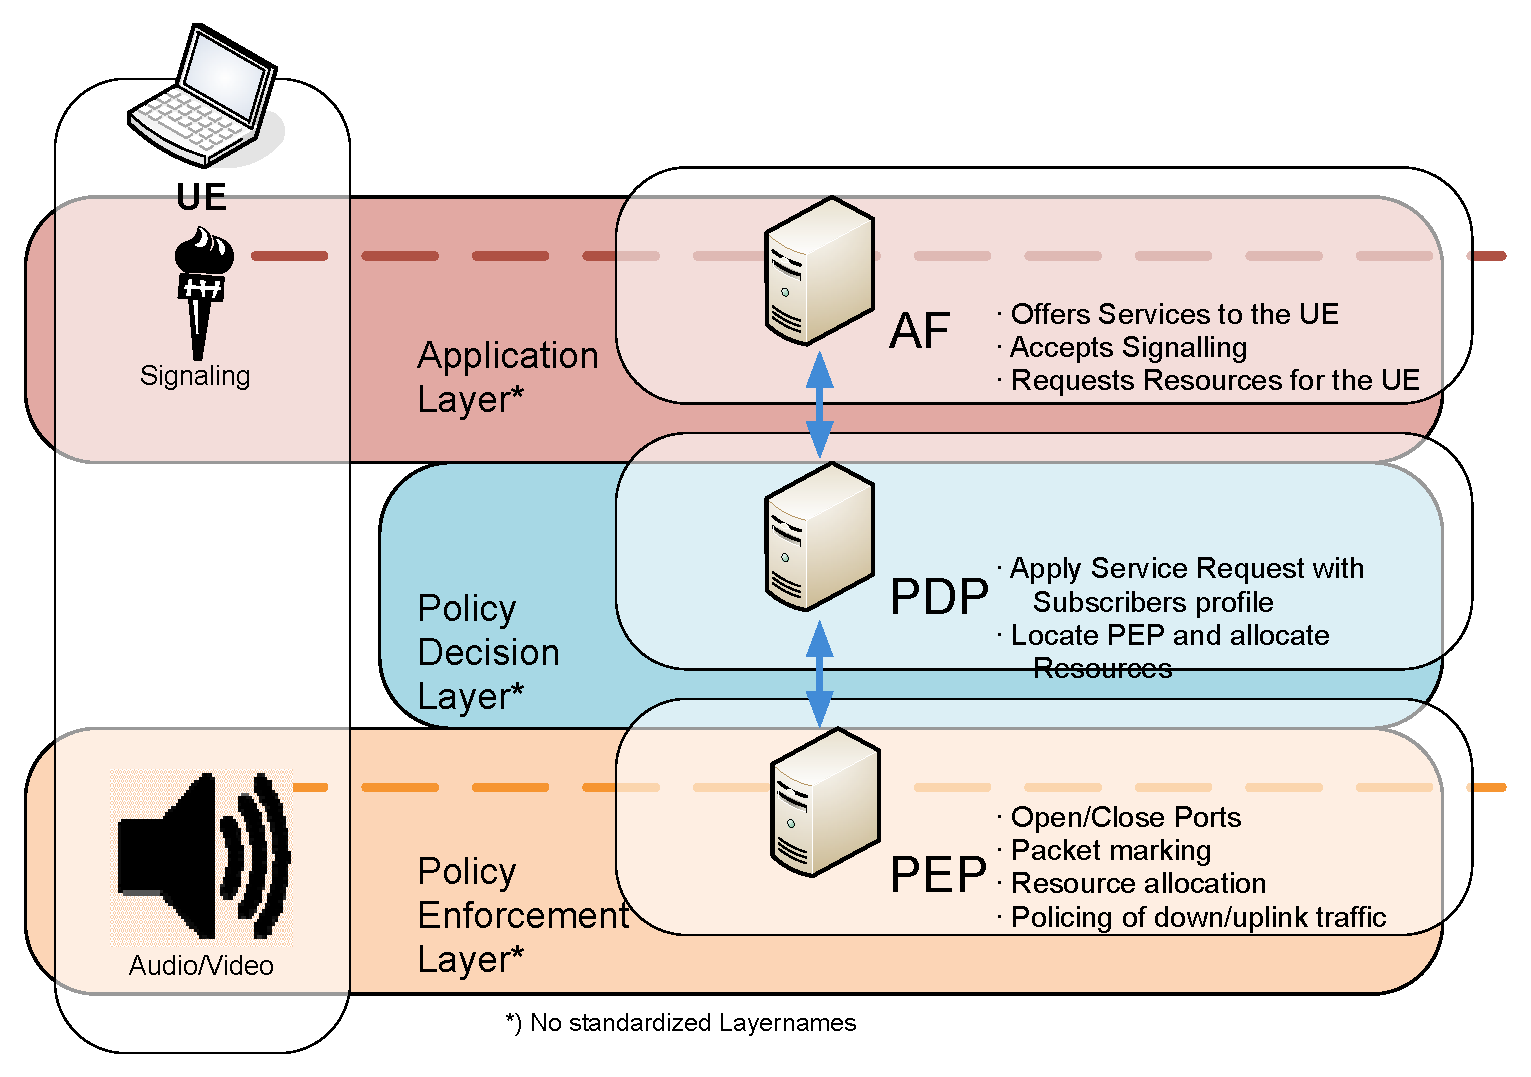
\includegraphics[width=\textwidth]{figures/IETFArch}
\end{center}
\caption{IETF Architecture of Policy-based Admission Control}
\label{fig:IETFArch}
\end{figure}

As far as NGN QoS enforcement is concerned, the standardization bodies 3GPP, (targeting mobile networks) and ETSI TISPAN (focusing on fixed NGN networks) have designed their own architectures, depending on the particular access network requirements. In the case of 3GPP, this architecture is called Policy and Charging Control (PCC) \cite{3gpp.23.203}. Figure \ref{fig:3GPPArch}	depicts main functions in this architecture which can be easily mapped to layers and functions in the previously presented IETF architecture.

\begin{figure}
\begin{center}
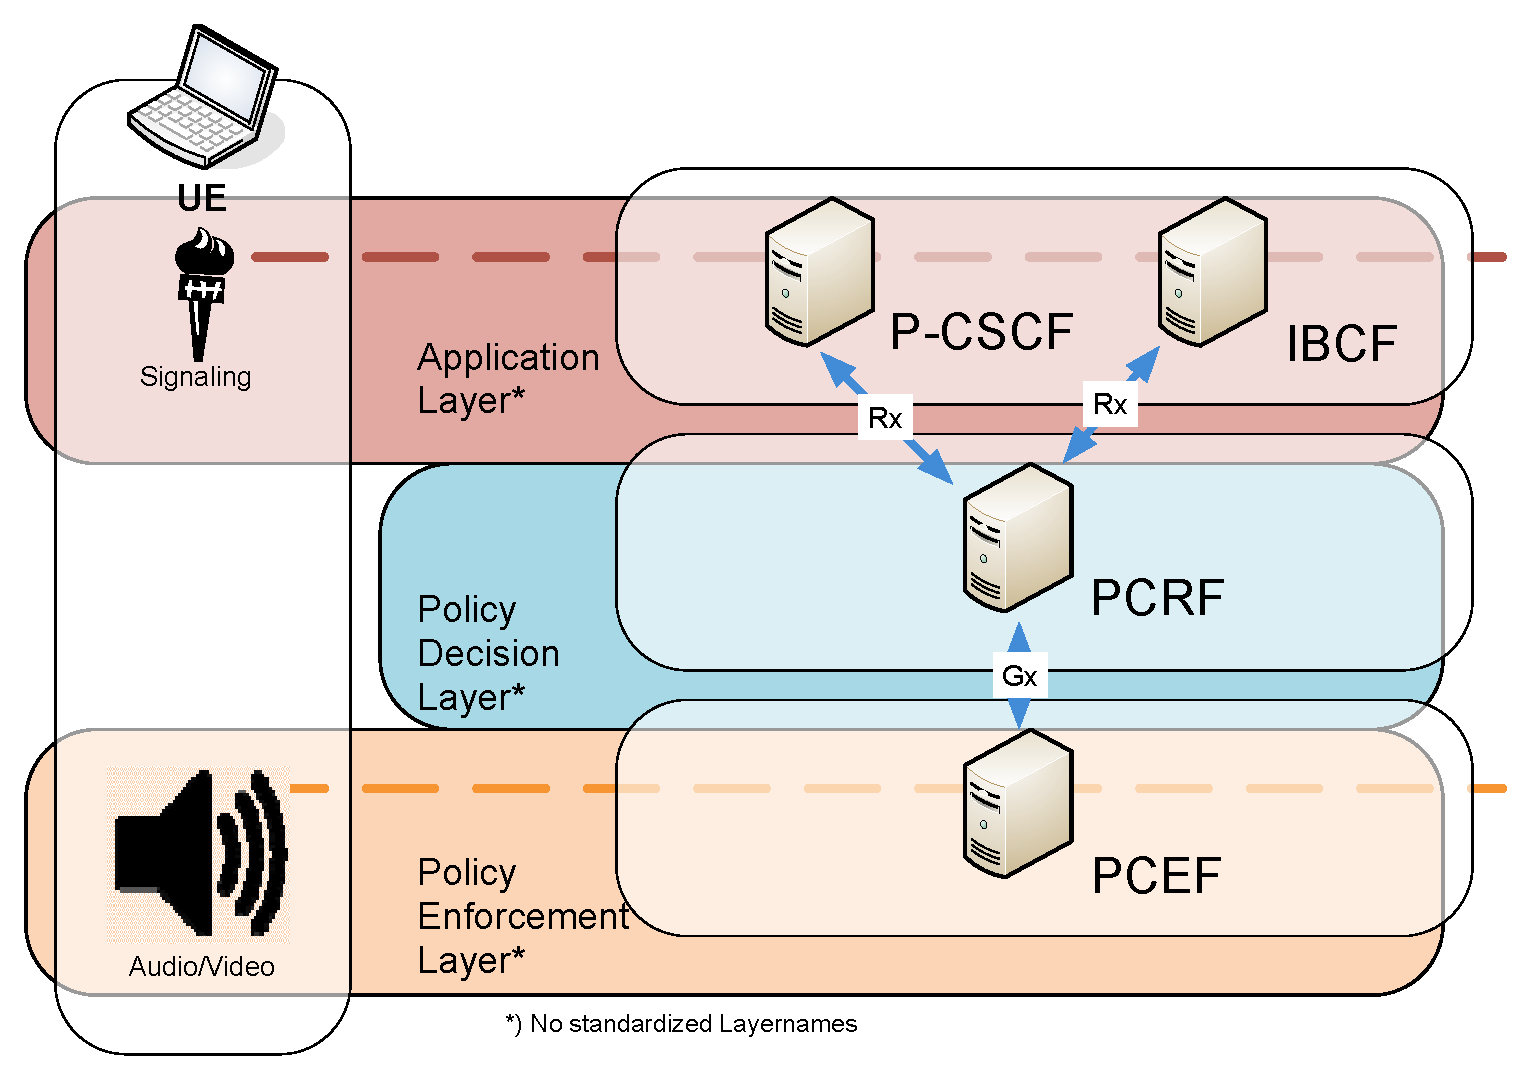
\includegraphics[width=\textwidth]{figures/3GPPArch}
\end{center}
\caption{3GPP PCC Architecture}
\label{fig:3GPPArch}
\end{figure}

On the other hand, as mentioned earlier, ETSI TISPAN has developed its own architecture for QoS enforcement which is called Resource and Admission Control Subsystem (RACS) \cite{etsi.282.003} and illustrated in Figure \ref{fig:ETSIArch}.

\begin{figure}
\begin{center}
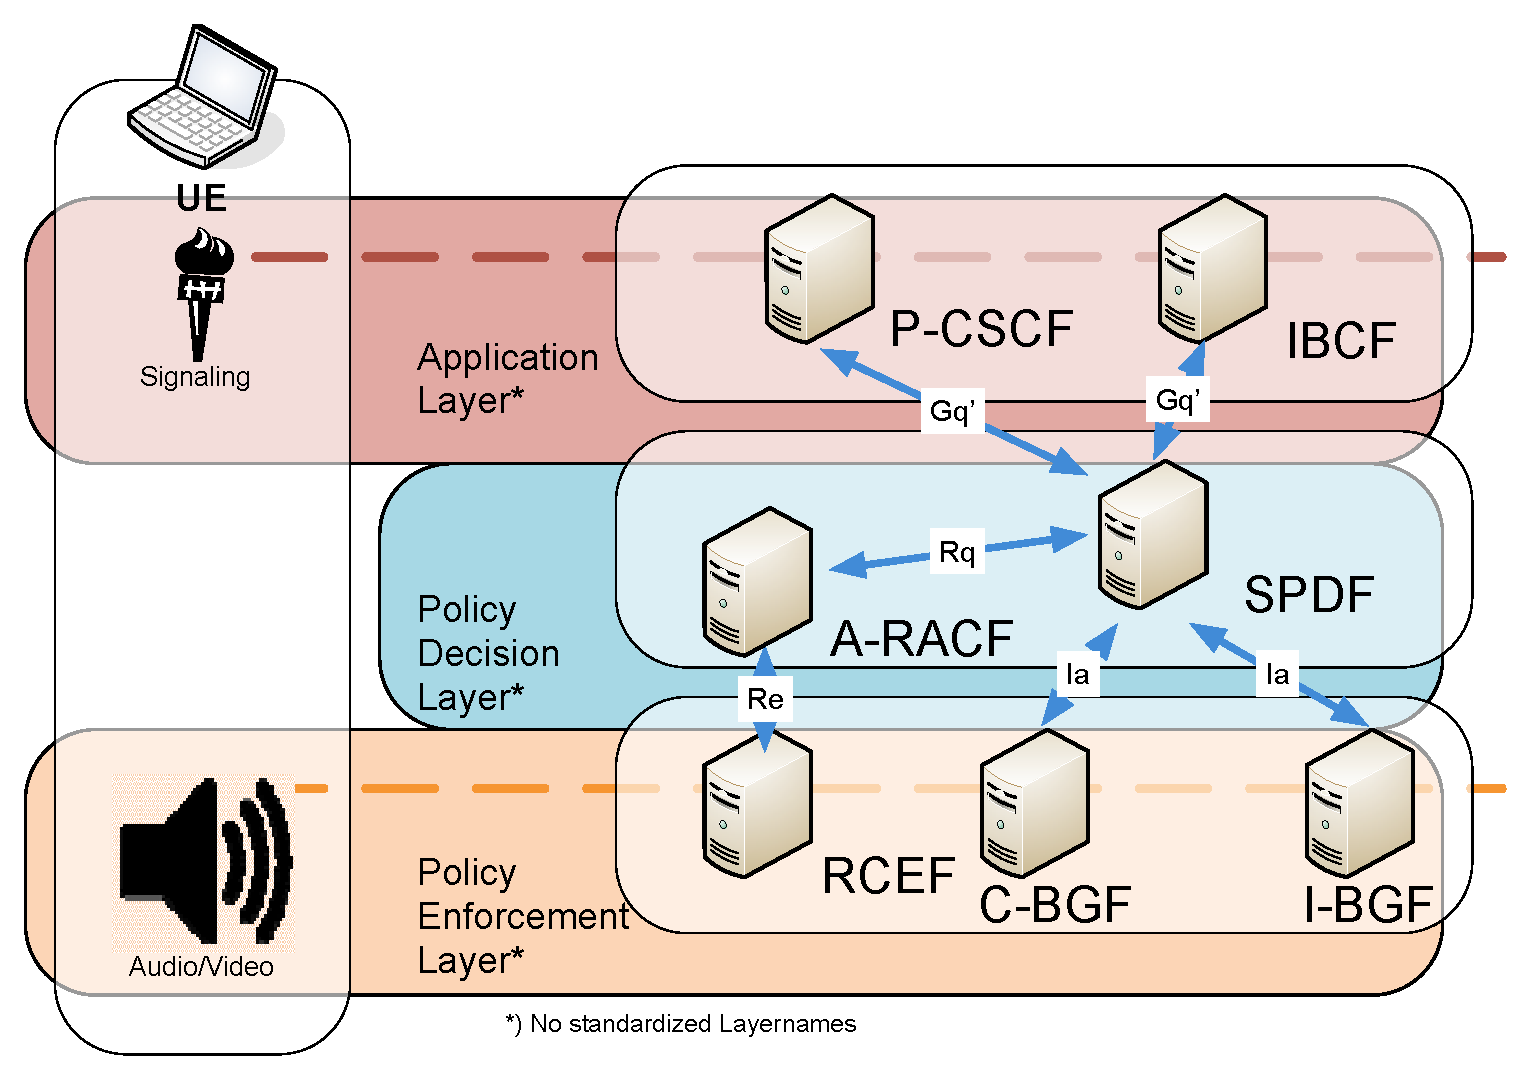
\includegraphics[width=\textwidth]{figures/ETSIArch}
\end{center}
\caption{ETSI TISPAN RACS Architecture}
\label{fig:ETSIArch}
\end{figure}

In order to merge these two architectural approaches into a common open source framework, BIQINI is heavily relying on advanced routing and traffic control tools provided by the open source operating system Linux, most notably several system tools which support IP traffic queueing configuration. A detailed description of routing, switching, bandwidth management, queuing and IP security functions in Linux systems can be found in \cite{website:lartc}, in the rest of this section we will only provide an in-depth view on the default Linux command-line application for queuing configuration which is called traffic control (tc) and supports the modification of the queuing strategies to be used for outgoing and incoming IP packets on specific network interfaces.

In tc, the different queuing types and --strategies are denoted as queuing disciplines. After setting up new queuing disciplines, IP packets must be assigned to certain queues using so-called filters which match the IP packets against specific patterns, corresponding to certain fields or byte sequences in the packet. Examples of these patterns include, e.g., source IP address, ports or any other field in the IP header. Upon successful match, the specific IP packet will be assigned to the corresponding queue. Note that a queuing discipline can, for instance, realize bandwidth management, reorder packets, delay packets, modify packets, etc., depending on the selected queuing discipline. A list of supported and implemented queuing algorithms can be found in \cite{website:lartc}.
The BIQINI implementation combines several queueing disciplines to realize QoS enforcement. The classful Hierarchical Token Bucket (HTB) algorithm manages the reserved bandwidth by allocating requested bandwidth to microflows. The queuing discipline dsmark manipulates the DSCP field of IP packets, marking all IP packets queued in a specific dsmark queue using a specified DSCP value.

BIQINI uses the queuing discipline netem for implementing realistic access network emulation. The netem algorithm can delay, reorder, drop, and duplicate IP packets. By setting up several netem queuing disciplines, with different delay and loss values for distinct DSCP marking emulates a DiffServ network.

Finally, selective rejection or dropping of IP packets can be configured using the ipTables \cite{website:netfilter} utility. A rule in ipTables describes traffic patterns and defines corresponding actions for this traffic, e.g., drop, reject, or accept. The traffic can be categorized by means of ports, addresses, protocol numbers, flags, etc. Similar to common firewalls, ipTables supports default rules for packets that cannot be matched to a rule. In most cases it is preferable to drop or reject all traffic that is not explicitly accepted by a rule.

\chapter{Architecture}
The basic architecture of the BIQINI implementation is sketched in Figure \ref{fig:BIQINIArch}. In the depicted scenario, the QoS enforcement is applied on an access link which on both ends is protected by respective PEPs. Whereas PEP 1 on the user side ensures that the micro-flow from the user agent to the core is scheduled correctly such that the service requirements (e.g. bandwidth) are fulfilled, PEP 2 on the core side is performing the same task for the opposite traffic direction. Note that, if PEP 1 were not installed, the user could use the access link excessively with other services, for instance sending extremely large emails or uploading huge amounts of data. Such bandwidth consuming services could then severely reduce the quality of realtime services like voice communication. Thus, PEP 1 ensures proper bandwidth usage in the uplink direction. This architecture is similar to \cite{etsi.182.031} which covers a study of enforcing QoS on Customer Premise Networks (CPN) and supports the realistic asymmetrical modeling of impairments on access links.

\begin{figure}
\begin{center}
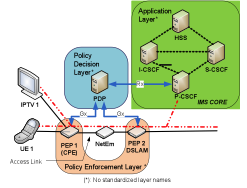
\includegraphics[width=\textwidth]{figures/BIQINI_ARCH}
\end{center}
\caption{Architecture of BIQINI QoS Enforcement for Access Links}
\label{fig:BIQINIArch}
\end{figure}


When no GGSN or DSLAM is available, the characteristics of a specific access network (e.g., ADSL or 3G) can be accurately emulated from the point of view of a layer 3 protocol with the NetEm instance depicted in Figure \ref{fig:BIQINIArch} \cite{jo:genericAccessEmu}. This is done by means of the Linux netem queueing discipline. 
In order to differentiate between different service classes, we also have installed a netem instance on the PEPs.
To be more specific, a microflow of the class "realtime conversational" needs low delay values and loss rates. In this case, our PEP has to guarantee that the service receives the correct QoS on the access link. To realize this, the PEP has to mark the IP packets with the correct DSCP value corresponding to this service class. As an example, we suggest to use the DSCP class 0x03 for realtime conversations. Thus, both PEPs have to mark packets of this class with the DSCP value 0x03, and at the same time the netem at the access link has to assign packets with DSCP value 0x03 to the queueing system handling realtime conversation, which, on its part, must realize low delay values and loss rates. On the other hand, best effort traffic could receive for instance the DSCP marking 0x00, which causes netem to treat such IP packets with a delay of several hundreds of msec and loss rates of 2\% and beyond.

In our overall QoS architecture, the PEPs are responsible for realizing bandwidth management. To this end, each incoming flow is shaped according to the installed rules. Flows that utilize too much bandwidth are queued at the PEP, thus increasing the corresponding delay value. In the worst case, this may lead to dropping the packets as soon as the queue is filled.

Our PEPs can be configured with or without ipTables (see section \ref{subsect:PEP}). In the case of a configuration without ipTables, any traffic is admitted but marked at the PEP as best effort traffic. Therefore, netem treats this traffic with lowest quality. However, if services are enforced through the PDP, they are marked at the PEP with a different ("better") DSCP value and are treated with higher priority. Additionally, the PEP also ensures that the enforced services can utilize their required bandwidth.

\begin{figure}
\begin{center}
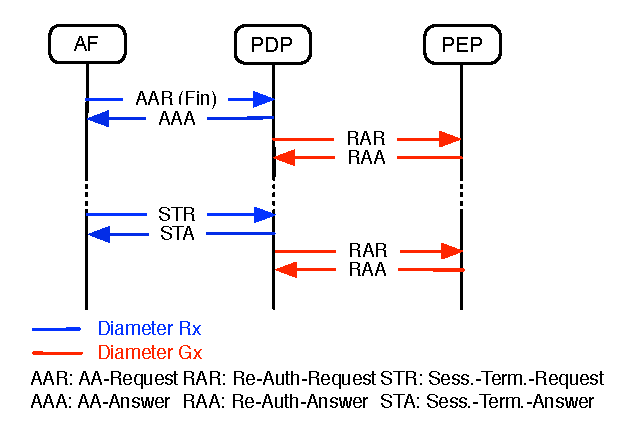
\includegraphics{figures/MsgFlowSetup}
\end{center}
\caption{Message Flow between AF, PDP and PEP}
\label{fig:flowsetup}
\end{figure}

The communication between AF, PDP and PEP is realized using the Diameter \cite{rfc3588} protocol. More specifically, the AF utilizes AA-Requests (AAR) and AA Answer (AAA) messages over the Rx interface \cite{3gpp.29.214} to transport authorization requests to the PDP, whereas the termination of a session is performed by a Session Termination Request (STR). The communication between PDP and PEP is realized over the Gx interface \cite{3gpp.29.212} and uses Re-AuthRequests (RAR) and Re-Auth Answer (RAA) messages. Figure \ref{fig:flowsetup} illustrates the Diameter messages employed.
%%%%%%%%%%%%%%%%%%%%%%%%%%%%%%%%%%%%%%%%%%%%%%%%%%

	\section{Components}
		\subsection{Policy Decision Point}
		As already mentioned previously, the PDP is the specific component that is responsible for translating the media-specific data of a service request (like codec and media type) to QoS-specific parameters (like bandwidth and delay requirements). In order to realize this task, the PDP uses rules from an external rules repository which allow deriving the appropriate QoS parameters from service specific and user specific data.
Our implementations of the Rx and Gx interfaces are based on the jDiameterPeer due to the Fraunhofer FOKUS group. On top of it we have built a basic logic which is able to handle incoming messages, to keep pointers to the corresponding state machines and to forward messages to the Rx and Gx interfaces. We have implemented the resulting state machine (depicted in Figure \ref{fig:statemachine}) as well as "dummy" interfaces to a Subscription Policy Repository (SPR) which handles user and domain policies. Additionally, our implementation provides references to the PEP instances which have to be used for each subscriber.
One of the main tasks of the PDP consists of mapping all requests to sessions, thus enabling the storage of a consistent state for each session. In this context, messages received by the Policy Decision Point (PDP) can be subdivided into preliminary service information messages and final service information messages. Whereas final service information messages install rules at the PEP, preliminary information messages only check if a requested service meets the corresponding policies and if there are enough resources available.
The resulting state machine includes therefore the following set of states:

\begin{itemize}
	\item Receiving: waiting for incoming AAR message
	\item Accepted PRE: received a AAR with Service-Type AVP set to \newline PRELIMINARY\_SERVICE\_INFORMATION
	\item Rejected: Service information received with not acceptable content (eitherdue to policy or insufficient resources)
	\item Accepted Final: received AAR with Service-Type AVP set to \newline FINAL\_SERVICE\_INFORMATION
	\item Committed: enforcing the rules at the PEP successful
	\item Closing: received STR from the AF, trying to terminate session at the PEP
	\item Failed: enforcing the rules at the PEP failed
	\item Terminated: Session successfully terminated
\end{itemize}

\begin{figure}
\begin{center}
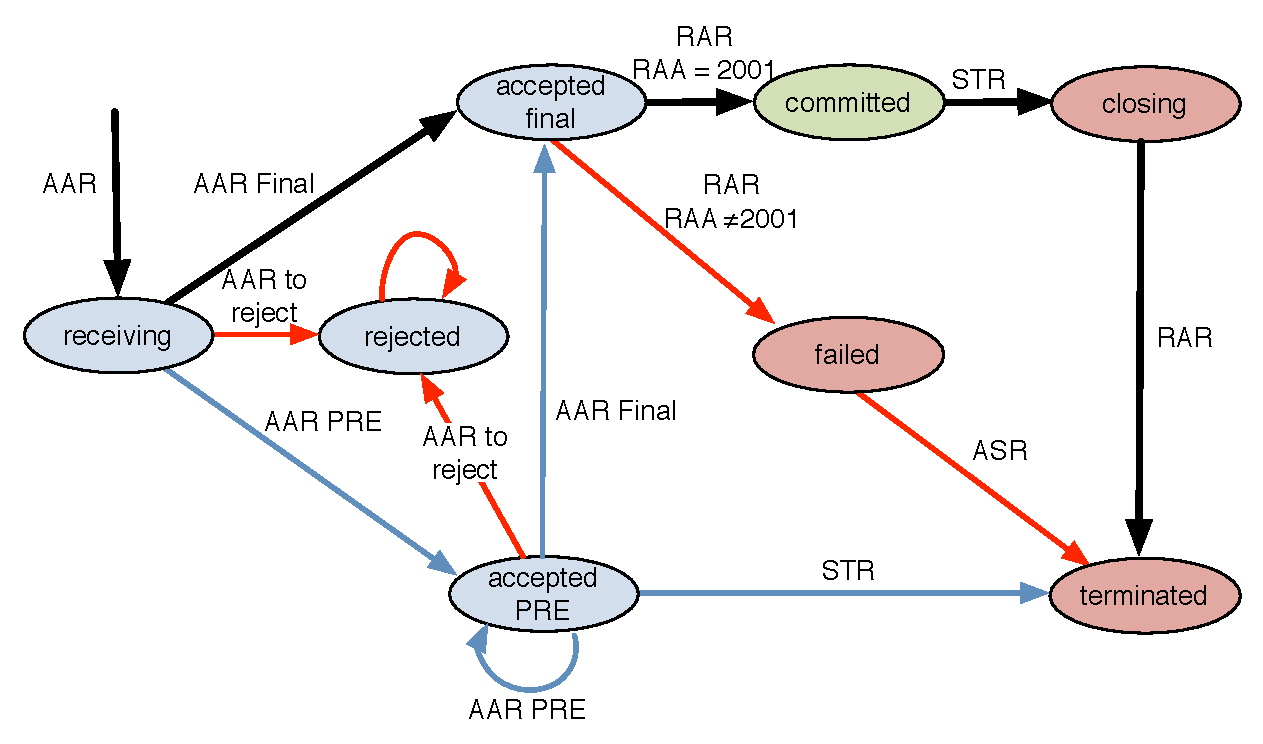
\includegraphics[width=\textwidth]{figures/StateMachine}
\end{center}
\caption{PDP State Machine}
\label{fig:statemachine}
\end{figure}


Note that in Figure \ref{fig:statemachine}, a sequence of black arrows depicts the traversal through the states, if the initial request already contains the final service information and if the installing of the rules at the PEP works properly. Blue arrows indicate that the initial request contains only preliminary service information, and a second request is sent to install the rules at the PEP. Red arrows are used if either the request coming from the AF is not acceptable or the installation of rules at the PEP has failed. In order to maintain the clarity of presentation, the three states necessary for a session update are not shown in the diagram. Note that for each session handled at the PDP, a new state machine is created in order to deal with the corresponding messages.
%%%%%%%%%%%%%%%%%%%%%%%%%%%%%%%%%%


		\subsection{Policy Enforcement Point}
		
		The Policy Enforcement Point (PEP) is responsible for detecting microflows and processing them according to the configured QoS parameters. Both processes (detection and processing) are defined by rules which are received via the Gx interface from the PDP.

\begin{figure}
\begin{center}
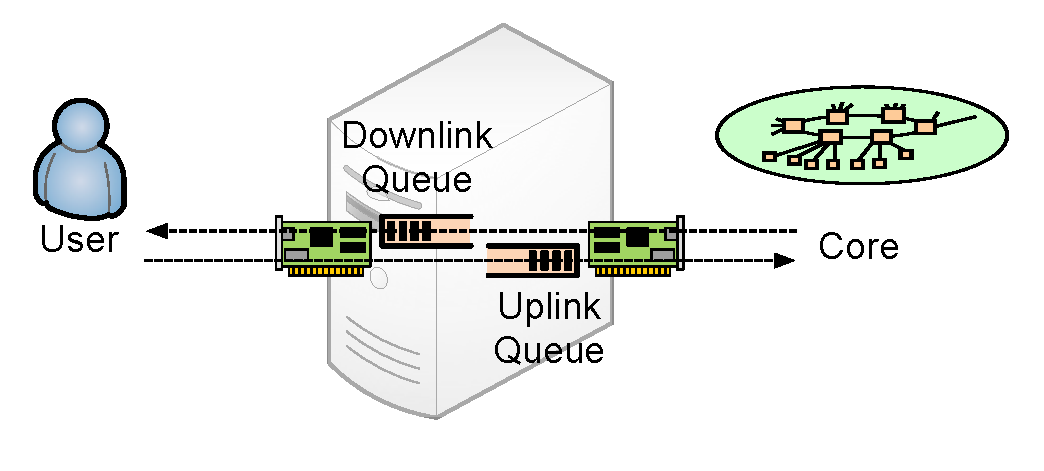
\includegraphics[width=\textwidth]{figures/PEPQueueing}
\end{center}
\caption{Interface Cards and Queueing at the PEP}
\label{fig:pepcards}
\end{figure}
		
		
Our implementation is realized with Java, reusing the jDiameter stack already introduced. The detection and enforcement process is realized by Linux tools like tc and ipTables. The PEP stores the current state and configuration of each rule and tracks the bandwidth consumption in the PEP Rules Management module. For a comprehensive illustration of the main PEP components we refer to Figure \ref{fig:pepcards}.
		
		
The PEP works an intermediate component between the communicating hosts. In order to be fully transparent for IP traffic, it is essential to configure the PEP as a bridge. With Linux, this requires two interface cards at the host, one towards the user agent and one towards the core network. The queueing is always realized at the sending interface, whereas QoS enforcement for traffic directed to the user agent can only be realized on the interface card towards the user agent (i.e. downlink). Similarly traffic directed to the core network can only be treated at the interface card towards the core network (i.e. uplink). In our implementation, we use the Linux system tool brctl to configure a Linux host with two interface cards as a bridge.
Additionally, we have decided to reuse the concepts for installing, modifying and removing of rules by means of the Diameter protocol from the 3GPP PCC architecture, where these rules are called "charging rules" and include four main aspects:

\begin{itemize}
	\item Each rule has a unique identifier (Charging Rule Name), which is mainly necessary to be able to remove a certain rule.
	\item Each rule is responsible for a certain microflow characterized by a flow description using the following parameters: source IP address, destination port, destination IP address and protocol number. In the case of a bidirectional flow, two such flow descriptions are required.
	\item The third part of a rule contains QoS information which is described in terms of the guaranteed bitrate, the maximally requested bandwidth and the traffic class (like streaming, realtime conversational, etc.). The traffic class is used to set the DSCP value properly.
	\item The last part in the charging rule concerns charging information. As our implementation currently does not consider any charging aspects, any information contained in this part is ignored.
\end{itemize}
Altogether, these four parts are encoded as so-called Charging Rule Definition AVPs, see Listing \ref{lst:chargRuleDef}.
\begin{lstlisting}[caption=Example of a Charging Rule Definition, label={lst:chargRuleDef}]
[Charging-Rule-Install] 
	[Charging-Rule-Definition]
		[Charging-Rule-Name]			Video-Rule;12345
		[Flow-Description]
			permit out 17 from 10.0.0.1 to 10.0.0.6 10001 
		[Flow-Description]
			permit in 17 from 10.0.0.6 to 10.0.0.1 3400
		[Flow-Status]				ENABLED (3)
		[QoS-Information]
			[QoS-Class-Identifier]		1
			[Max-Requested-Bandwidth-UL]	17500
			[Max-Requested-Bandwidth-DL]	17500
			[Guaranteed-Bitrate-UL]		15000
			[Guaranteed-Bitrate-DL]		15000
		[Online]				DISABLE\_ONLINE (0)
		[Offline]				ENABLE\_OFFLINE (1)
		[Metering-Method]			DURATION (0)
		[AF-Charging-Identifier]		chargingid987654321 
\end{lstlisting}

After starting the PEP, some generic rules have to be installed first (for example signaling traffic should be able to pass under all circumstances). Such predefined rules are stored in the configuration file of the PEP and are activated automatically. As an alternative option, these rules can also be installed by a Charging Rule Command triggered by the PDP.
After receiving an installation request via the Gx interface, the PEP has to configure the bandwidth management (realized with the HTB queueing discipline) and activate the firewall for the respective microflow. The rate and ceil parameters of the tc command are configured by the guaranteed bitrate and Max- Requested Bandwidth value of the QoS Information AVP, which has to be completed both for the uplink and downlink direction in the case of a bidirectional microflow. To realize DiffServ marking, we add a dsmark queueing discipline and configure a DSCP value that fits to the traffic class. In the next step, the firewall is informed by the ipTables command that this microflow has to be allowed to pass through. As mentioned before, it is also possible to run the PEP without gate blocking. By using the tc queuing system HTB, it is guaranteed that a certain microflow cannot exceed the reserved maximum requested bandwidth. If too much traffic should be injected into the network, the PEP will shape the traffic according to the installed rules. Additionally, the currently used bandwidth and the total amount of sent bytes are observed for each microflow. These data could be used in later releases to realize flow-based charging. Note that we do not use these data to infer a bearer loss, as individual services could generate traffic patterns with no data sent over a long period of time that would wrongly be detected as bearer loss.
		
		
		\subsection{Application Function}
		Wer?
	\section{Interaction}
		(TS 32.XXX)
		Wer?
		
		
		
\chapter{Configuration}
	\section{Prerequisites}
	For a computer to run BIQINI, the following tools have to be installed:
	\begin{itemize}
		\item ant
		\item Java 1.6
		\item traffic control
		\item iptables
	\end{itemize}
	As the enforcing part uses TC and iptables, the PEP has to be run on a Linux machine.
	The PDP runs on any other operating system running Java 1.6.

	\section{Set-Up}
		After downloading the zip file, it must be extracted which gives us multiple folders:
		\begin{itemize}
			\item bin: destination for compiled binaries
			\item cfg: configuration files
			\item doc: this documentation
			\item lib: library folder for external libraries, e.g., log4j
			\item src: source folder
		\end{itemize}
		
		\subsection{Compiling}
			The extracted files also include a build file for ant, build.xml.
			To compile, spawn a shell, move to the folder where the files were extracted and type "ant".
			If all prerequisites are met, ant uses the Java compiler to build the sources and copies them to "bin".
		
	\section{System Set-Up}
		The folder "cfg" comes with some configuration examples, this section shows how to use and modify them for a specific scenario.
		The following sections show the configuration for each part.
		\subsection{Policy Decision Point}
		The PDP comes with three distinct configuration files which have the following purpose:
\begin{itemize}
	\item Diameter peer configuration
	\item PEP settings
	\item Bandwith settings for codecs
\end{itemize}
%%%%%%%%%%%%%%%%%%%%%%%%%%%
\subsubsection{Diameter peer configuration}
As this implementation uses the JavaDiameterPeer implementation from Fraunhofer FOKUS, the peer configuration is done as stated within \cite{website:javaDiameterPeer}.

An example is depicted within Listing \ref{lst:DiamPeerCfg}.

\lstset{language=xml,keywords={DiameterPeer,Acceptor,Auth,Acct,Peer},emph={FQDN, Realm, Vendor_Id, Product_Name, AcceptUnknownPeers, DropUnknownOnDisconnect,id,vendor},keywordstyle=\color{red},emphstyle=\color{blue}}
\begin{lstlisting}[caption=Example of a Diameter Peer configuration file, label={lst:DiamPeerCfg}]
<?xml version="1.0" encoding="UTF-8"?>
<DiameterPeer
		FQDN="pdp.open-ims.test" 
		Realm="open-ims.test" 
		Vendor_Id="10415" 
		Product_Name="JavaDiameterPeer">
	<Acceptor port="3868"/>
	<Auth id="16777216" vendor="10415"/>
	<Auth id="16777216" vendor="0" />
	<Acct id="16777216" vendor="0" />
	<Peer FQDN="pcscf.open-ims.test" Realm="open-ims.test"/>
	<Peer FQDN="pep1.open-ims.test" Realm="open-ims.test"/>
	<Peer FQDN="pep2.open-ims.test" Realm="open-ims.test"/>
	<Auth id="16777236" vendor="10415"></Auth>
	<Acct id="16777236" vendor="10415"></Acct>
	<Auth id="16777236" vendor="0"></Auth>
	<Acct id="16777236" vendor="0"></Acct>
</DiameterPeer>
\end{lstlisting}

All PEPs, which shall be used for enforcement, must be inserted here as Diameter Peers!
See also next section for details.



%%%%%%%%%%%%%%%%%%%%%%%%%%%%%%%%%%%%%%%%%%%%%%%%
\subsubsection{PEP settings}
This file tells the PDP which PEPs it shall use for which user and how much bandwidth each PEP has available.
Listing \ref{lst:PEPContainer} shows an example.

\lstset{language=xml,keywords={PEPContainer,PEP,User},emph={ip,domain,upbw,dobw},keywordstyle=\color{red},emphstyle=\color{blue}}
\begin{lstlisting}[caption=Example of a PEP settings file, label={lst:PEPContainer}]
<?xml version="1.0" encoding="UTF-8"?>
<PEPContainer>
	<PEP ip="10.10.1.1" domain="open-ims.test" upbw="200000" dobw="200000">
	<!--pep1.open-ims.test-->
		<User ip="10.10.2.1"/>
		<User ip="10.10.2.2"/>
		<User ip="10.10.2.3"/>
	</PEP>
	<PEP ip="10.10.1.2" domain="open-ims.test" upbw="200000" dobw="200000">
	<!--pep2.open-ims.test-->
		<User ip="10.10.2.1"/>
		<User ip="10.10.2.2"/>
		<User ip="10.10.2.3"/>
	</PEP>
</PEPContainer>
\end{lstlisting}
This example shows a PDP enforcing at two PEPs at "10.10.1.1" as well as "10.10.1.2" for the users at "10.10.2.X".
Each of them has a total bandwith of 200 KBit per second for all users.

All PEPs, configured within this file have to be in the Diameter peer configuration file as "Peer".
%%%%%%%%%%%%%%%%%%%%%%%%%%%%%%%%%

\subsubsection{Bandwith settings for codecs}
Within the file "codebook.xml", bandwith parameters of used codecs can be set.
Listing \ref{lst:codebook} shows details.

\lstset{language=xml,keywords={codecs,codec},emph={encodingName,payloadType,type,bandwith},keywordstyle=\color{red},emphstyle=\color{blue}}
\begin{lstlisting}[caption=Example of a PEP settings file, label={lst:codebook}]
<?xml version="1.0" encoding="UTF-8"?>
<codecs>
   <codec encodingName="PCMU" payloadType="0" type="audio" bandwidth="87200"/>
   <codec encodingName="GSM" payloadType="3" type="audio" bandwidth="29200"/>
   <codec encodingName="H263" payloadType="34" type="video" bandwith="500000"/>
   <codec encodingName="H263-1998" type="video" bandwidth="500000"/>
</codecs>
\end{lstlisting}
The parameters have the following meaning:
\begin{itemize}
	\item encodingName: the name of the codec as used within the SDP payload
	\item payloadType: default type value as used within SDP (optional)
	\item type: can be audio or video
	\item bandwith: needed bandwith, inclusive all overhead
\end{itemize}




		\subsection{Policy Enforcement Point}
		\label{subsect:PEP}
		The PEP needs two configuration files for the following purpose:
\begin{itemize}
	\item Diameter peer configuration
	\item Enforcement settings
\end{itemize}
A major perquisite of the PEP is the correct interface configuration.
This is described in the next section.
%%%%%%%%%%%%%%%%%%%%%

\subsubsection{Interface configuration}
The system needs at least two interface cards, one for the user and one for the core side. 
These interface cards should not have IP addresses assigned, but should be configured as bridge by means of the bridge control tool (brctl). Afterwards the bridge has to be configured with an IP address where the PDP can send its requests to.

The following script does the neccessary configuration:

\begin{lstlisting}[caption=Example of a PEP Enforcement Setting, label={lst:PEPBridgeConf}]
#!/bin/sh

#Remove the IP addresses
sudo ifconfig eth0 0.0.0.0
sudo ifconfig eth1 0.0.0.0

#Create a bridge
sudo brctl addbr bridge

#Add interfaces to the bridge
sudo brctl addif bridge eth0
sudo brctl addif bridge eth1
 
#Configure an IP address  for the bridge
sudo ifconfig bridge x.x.x.x netmask y.y.y.y

#Bring up the bridge interface
sudo ifconfig bridge up
\end{lstlisting}

%%TODO more details and references

\subsubsection{Diameter peer configuration}
The configuration of the PEP Diameter stack follows the guidelines of the PDP section, with minor modifications. The PEP is awaiting the connection from the PDP, so we do not need to configure the diameter peer parameters of the PDP.

The following example fulfills all requirements:

\lstset{language=xml,keywords={DiameterPeer,Acceptor,Auth,Acct,Peer},emph={FQDN, Realm, Vendor_Id, Product_Name, AcceptUnknownPeers, DropUnknownOnDisconnect,id,vendor},keywordstyle=\color{red},emphstyle=\color{blue}}
\begin{lstlisting}[caption=Example of a Diameter Peer configuration file, label={lst:DiamPeerCfgPEP}]
<?xml version="1.0" encoding="UTF-8"?>
<DiameterPeer
		FQDN="pep.open-ims.test" 
		Realm="open-ims.test" 
		Vendor_Id="10415" 
		Product_Name="JavaDiameterPeer">
	<Acceptor port="3868"/>
	<Auth id="16777216" vendor="10415"/>
	<Auth id="16777216" vendor="0" />
	<Acct id="16777216" vendor="0" />
</DiameterPeer>
\end{lstlisting}
%%%%%%%%%%%%%%%%%%%%%

\subsubsection{Enforcement settings}
In this part we explain the settings of the QoS enforcement part at the PEP, what is also done within an XML file. 
This file has two parts, one for general settings, and one for predefined rules, that can be activated at startup of the PEP, or later through the PDP.

\lstset{
	language=xml,
	keywords={pep-rule-config,common-config,predefined-rules,gateblocking,queuesize,logging,CommandExecution,interface,DSCP_mapping,unclassified-traffic, bandwidthUsageLogging, entry,expires, rule, uplink, downlink,TC_IDs },
	emph={blockallGates, enable, size, count, info, diameterMessages, emulate, name, bandwidth, direction, QCI, DSCP, debug, defaultid, startid, stopid, min, max, intervall, supported, automatic, timeout, active, GuaranteedBitrate,MaxRequestedBandwidth},
	keywordstyle=\color{red},
	emphstyle=\color{blue},
	alsodigit={-}
	}

The PEP blocks all unclassified traffic, when the following configuration is used:
\begin{lstlisting}[caption=Activation of Gateblocking, label={lst:PEPGate}]
	<gateblocking blockallGates="true"/>
\end{lstlisting}
To allow unclassified traffic blockallGates has to be changed to false.

The capacity of the queues of the queueing systems on the uplink and downlink interfaces can be configured by means of bytes or packets.
The following example illustrates a queue which stores up to 100kBytes.
\begin{lstlisting}[caption=Queue with 100kBytes, label={lst:PEPContainer}]
	<queuesize enable="true" size="100000" count="bytes"/>
\end{lstlisting}
The next listing depicts a queue which can store up to 100 packets
\begin{lstlisting}[caption=Queue with 100 packets, label={lst:PEPContainer}]	
	<queuesize enable="true" size="100" count="packets"/>
\end{lstlisting}

The next setting configures the logging, which is sent to the console.
The info setting logs actions that are performed at the PEP, the diameterMessages setting logs the arrival and departure of diameter messages.
\begin{lstlisting}[caption=Enable Logging, label={lst:PEPContainer}]	
	<logging info="true" diameterMessages="true"/> 
\end{lstlisting}

The PEP can also be used as 'dummy' on an arbitrary system (e.g., when not enough interface cards are available and/or the operating system is not Linux).
The setting emulate="true" prevents the PEP from executing system calls, what is e.g., useful for debugging.
The setting debug="true" prints all system commands to the console.
\begin{lstlisting}[caption=Enable Emulation, label={lst:PEPContainer}]	
	<CommandExecution emulate="true" debug="true"/>  
\end{lstlisting}

The following settings configure the interfaces to be used for uplink (in) and downlink (out) direction, as well as for the absolute assigned bandwidth.
The interface names have to be the names given in the system, e.g.,  eth0 or eth1.
\begin{lstlisting}[caption=Interface configuration, label={lst:PEPContainer}]	
	<interface name="eth1" bandwidth="10M" direction="in"/>  
	<interface name="eth0" bandwidth="10M" direction="out"/>  
\end{lstlisting}

The PEP is able to mark the packets by means of DSCP. This marking depends on the QCI parameter from the PDP. 
The section DSCP\_mapping stores a translation from QCI values to DSCP marks. 
For example the following snap illustrates a mapping where streams with the QCI value of 1 are marked with 0x12 in the DSCP filed and with 0xFF if the stream belongs to a QCI  value of 2.
\begin{lstlisting}[caption=DSCP mapping, label={lst:PEPContainer}]	
	<DSCP_mapping>
		<entry QCI="1" DSCP="0x12"/>
		<entry QCI="2" DSCP="0xFF"/>
	</DSCP_mapping>
\end{lstlisting}

The TC\_IDs describe the queue ids for the default queue and the dynamically installed queues. Theses values should not be changed. In rare cases, where more then 450 parallel streams are handled, it might be a good idea to increase the stopid value.
\begin{lstlisting}[caption=TC ids, label={lst:PEPContainer}]	
	<TC_IDs defaultid="7000" startid="7100" stopid="8000" />
\end{lstlisting}

The setting unclassified-traffic sets the maximum bandwidth allocation to traffic that can not be mapped to a rule. 
The min and max parameter represent the minimal guaranteed bitrate and the maximal bitrate for unclassified traffic. 
The following example configuration line sets a bitrate of 5kbit/sec up to 20kbit/sec for unclassified traffic. 
Only integers are allowed for describing the bitrate. So 1600k is allowed to describe 1600 kBit/sec, whereas 1.6M will not be accepted by the parser. 
\begin{lstlisting}[caption=Bitrates for unclassified traffic, label={lst:PEPContainer}]	
	<unclassified-traffic min="5k" max="20k"/>
\end{lstlisting}

The PEP allows to observe the current used bandwidth. 
The following configuration line sets the interval for measuring the current bandwidth usage of each single stream.
\begin{lstlisting}[caption=bandwidth usage intervall logging, label={lst:PEPContainer}]	
	<bandwidthUsageLogging intervall="1sec"/>
\end{lstlisting}

The expire configuration (experimental!) describes the maximum duration of a rule when soft state configuration is used. 
Rules that are not updated within this time are automatically deleted. 
\begin{lstlisting}[caption=expires configuration, label={lst:PEPContainer}]	
	<expires supported="false" automatic="true" timeout="2min"/>
\end{lstlisting}

In the following section we describe predefined rules, which are configured after startup of the PEP. 
These rules can be activated immediately (active="default") or only be configured and activated later by the PDP (active="ready").

The next configuration line illustrates a predefined rule for SIP traffic, named SIP.
\begin{lstlisting}[caption=predefined rule for SIP, label={lst:PEPContainer}]	
<rule name="sip" QCI="1" active="ready">
	<uplink GuaranteedBitrate="100k" MaxRequestedBandwidth="500k">
		permit in ip from 0.0.0.0 to 0.0.0.0 5060
	</uplink>
	<downlink GuaranteedBitrate="100k" MaxRequestedBandwidth="500k">
		permit out ip from 0.0.0.0 5060 to 0.0.0.0
	</downlink>
</rule>	
\end{lstlisting}

In this rule we assign the QCI value of 1 to all IP packets that follow the same patterns as described below. 
The keyword default indicates that this rule is activated after startup.
The guaranteed bit rate, which is always reserved for this stream, is configured with separate lines for uplink and downlink. 
MaxRequestedBandwidth is the bandwidth that this stream can use maximal, but this is not guaranteed. 
Within each downlink and uplink line is the ipfilter rule that describes the pattern of the ip traffic that belongs to this rule.

We hardly recommend to configure at least rules for SIP, Diameter and DNS. 
Only in cases where it is clear that non of these protocols traverse the PEP, the rules should be removed. 
In scenarios, where two PEPs are used and Diameter rules are not activated, the Diameter traffic is handled as unclassified traffic and has to compete with other unclassified traffic.
In cases where UDP is used for unclassified traffic, the diameter traffic will starve and no communication to the PEP is possible anymore.

The following listing summarizes all configuration lines.
\begin{lstlisting}[caption=Example of a PEP Enforcement Setting, label={lst:PEPContainer}]
<?xml version="1.0" encoding="UTF-8"?>
<pep-rule-config>
  <common-config>
    <gateblocking blockallGates="false"/>
    <queuesize enable="true" size="100000" count="bytes"/>
    <logging info="false" diameterMessages="true"/>
    <CommandExecution emulate="true" debug="true"/>  
    <interface name="eth1" bandwidth="10M" direction="in"/>  
    <interface name="eth0" bandwidth="10M" direction="out"/>  
    <DSCP_mapping>
      <entry QCI="1" DSCP="0x12"/>
      <entry QCI="2" DSCP="0xFF"/>
    </DSCP_mapping>
    <TC_IDs defaultid="7000" startid="7100" stopid="8000" />
    <unclassified-traffic min="5k" max="20k"/>
    <bandwidthUsageLogging intervall="1sec"/>
    <expires supported="false" automatic="true" timeout="2min"/>
  </common-config>

  <predefined-rules>
  <rule name="ssh" QCI="1" active="ready">
    <uplink GuaranteedBitrate="1M" MaxRequestedBandwidth="1.1M">
      permit in 6 from 0.0.0.0 to 0.0.0.0 22
    </uplink>
    <downlink GuaranteedBitrate="1M" MaxRequestedBandwidth="1.1M">
      permit out 6 from 0.0.0.0 22 to 0.0.0.0
    </downlink>
  </rule>
  <rule name="sip" QCI="1" active="default">
    <uplink GuaranteedBitrate="100k" MaxRequestedBandwidth="500k">
      permit in ip from 0.0.0.0 to 0.0.0.0 5060
    </uplink>
    <downlink GuaranteedBitrate="100k" MaxRequestedBandwidth="500k">
      permit out ip from 0.0.0.0 5060 to 0.0.0.0
    </downlink>
  </rule>
  <rule name="diameter" QCI="1" active="default">
    <uplink GuaranteedBitrate="100k" MaxRequestedBandwidth="500k">
      permit in ip from 0.0.0.0 to 0.0.0.0 3868
    </uplink>
    <downlink GuaranteedBitrate="100k" MaxRequestedBandwidth="500k">
      permit out ip from 0.0.0.0 3868 to 0.0.0.0
    </downlink>
  </rule>
  <rule name="dns" QCI="1" active="default">
    <uplink GuaranteedBitrate="10k" MaxRequestedBandwidth="200k">
      permit in 6 from 0.0.0.0 to 0.0.0.0 53
    </uplink>
    <downlink GuaranteedBitrate="10k" MaxRequestedBandwidth="200k">
      permit out 6 from 0.0.0.0 53 to 0.0.0.0
    </downlink>
  </rule>
</predefined-rules>
</pep-rule-config>
	
\end{lstlisting}

The PEP can be started with the following command line. 

\begin{lstlisting}[caption=Example of a PEP Enforcement Setting, label={lst:PEPContainer}]
sudo java -jar PEP.jar diameter_cfg.xml pep_rule_config.xml
\end{lstlisting}

\subsubsection{Common problems}
The following section describes problems and pitfalls we had during our tests.
Some configuration parameters are often the root of misconfiguration and unexpected behavior. 
In these cases we recommend to activate all logging and to read the responses carefully. We summarize here some common known misconfigurations.

\begin{itemize}
	\item Please ensure that you provide both configuration files and that you run the application as root. 
	The PEP configures queueing disciplines and firewall settings what requires root privileges.

	\item After starting the application, it is possible to change the configured logging or to observe the active rules and their current as their consumed bandwidth.
	
	\item In the case that all rules are successfully received and a successful response was sent back, but the enforcement does not work correctly as expected, make sure that the PEP application was started as root and the PEP was able to configure the tc and IPtable commands. If the application has no root privileges the application can not modify queueing and firewall parameters.

	\item If the application has the correct privileges and the enforcement works properly, but the application does not show any traffic through the rules, or traffic which passes is marked as unclassified traffic, whereas the patterns as IP addresses and ports are correct. The most common reason for this problem is that the uplink and downlink interface names are swapped.

	\item In cases where the rule is installed, but no rule or only some rules are found in the active rule list, please read the diameter response message carefully and check the free bandwidth. 
	The most likely reason for this problem is insufficient free bandwidth. 
	Another reason might be that the PDP requests only uplink or downlink rules.

	\item If the PEP introduces too much delay for the traffic, the reason might be that the current usage is higher than the reserved or max requested bandwidth. 
	Check the current bandwidth usage and reconfigure your PDP. 
	High delays can also be an indication for a too long queue.
	Shorter queues lead to higher drop rates, but lower delay values.
	Note the current implementation allows no separate queuelength configuration for different QCI classes and bandwidth, so that the maximum delay can be configured through the QCI class.
\end{itemize}
%Marco bitte ins File PEP.tex deine Ausf�hrungen schreiben!
		\subsection{Application Function}
		Wer macht das?
	\section{Typical Scenarios}
	Marco \& Christoph
\bibliographystyle{plain}	% (uses file "plain.bst")
\bibliography{references,rfc,3gpp,i-d}

\end{document}